\documentclass[a4paper,titlepage,11pt]{article}

% \usepackage[top=2.54cm, bottom=2.54cm, left=2.54cm, right=2.54cm]{geometry}
\usepackage[utf8x]{inputenc}
\usepackage{hyperref}
\usepackage{graphicx}
\usepackage{hyperref}
\usepackage{multicol}
\usepackage{textcomp, xspace}

\begin{document}

\begin{titlepage}
  \begin{center}
    {\scshape \huge Schelling's Model of Segregation \par}
    \vspace{1cm}

    {\scshape \LARGE Project \par}
    \vspace{1.5cm}

    {\scshape \Large Complex Network \par}
    \vspace{0.5cm}

    {\Large Alameda \par}
    \vfill

    {\itshape \Large Group 6 \par}
    \vfill

    \begin{tabular}{l l}
      Bernardo Casaleiro & 87827\\
      João Godinho & 87830\\
    \end{tabular}
    \vfill

    {\large \today\par}
  \end{center}
\end{titlepage}

\section{Introduction}
Thomas Schelling is an American economist and professor at the School of Public Policy at University of Maryland.
In 1971 he created an agent-based model to help explain how segregation emerges and why is it so difficult to combat.
This model has the purpose of studying the segregation of races over time showing that even when agents don't mind
being surrounded by agents of a different race, they will yet segregate themselves from other agents over time.

For this project we replicated and analyzed the Schelling's Model. Our main goal was to discover the threshold
where agents are confortable with other races in their neighborhood and the end result of this variable.

We decided to continue to use the same language as our first project. So we used \href{https://www.python.org}{Python}.
To build the interface we used \href{https://wiki.python.org/moin/TkInter}{Tkinter},
and to draw the graphs (contour plot) we used \href{https://plot.ly/}{plotly}.

\newpage

\section{Implementation}
At the start a matrix is initialized and populated with all the agents and empty spots.
This will be the matrix where all the operations will happen.

Then we enter a simple iterative cycle that runs until either all the agents reach the goal satisfaction
\footnote{Satisfaction: An agent has a lower and upper boundary that establish the minimum and maximum
percentage of agents with his race in the neighborhood. If this limits are respected the agent is considered
satisfied.}
or a barrier is reached and it is not possible to satisfy all agents. 
This cycle has 3 steps:

\begin{description}
\item [ Calculate Satisfaction ] Calculates the satisfaction for every agent and return a list with all the unsatisfied ones.
\item [ Calculate Empty Spaces ] Returns a list of all the empty spaces.
\item [ Move the Unsatisfied agents ] Moves all the unsatisfied agents to one of the empty spaces available.
\end{description}

\subsection{Heuristics}
There were three heuristics implemented: Random, Best, Closest.

\subsubsection{Random}
The agent is randomly placed on an empty space available.

\subsubsection{Best}
The satisfation of the agent is calculated for each empty space.
Placing the agent in the empty space that provides the best fit.

\subsubsection{Closest}
The agent is placed on the closest empty space.
In order to avoid that an agent is always switching between two spaces,
each agent has a memory that keeps track of the last empty space he has been to.

\newpage

\subsection{Variables}
In our interface is possible to change all variables necessary to run the simulation:

\begin{figure}[h]
    \centering
    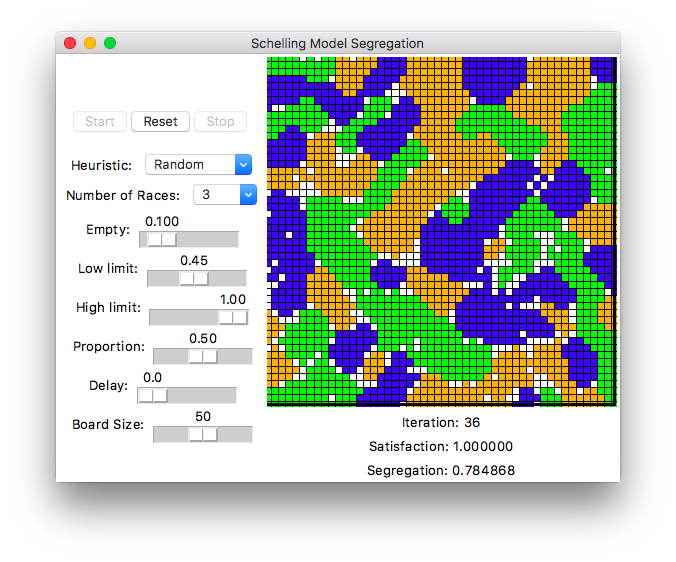
\includegraphics[scale=0.50]{img/interface.png}
\end{figure}

\begin{description}
\item [ Heuristic ] (Random or Best or Closest) \textbf{-} heuristic used for simulation
\item [ Number of Races ] (2 or 3) \textbf{-} number of races there will exist
\item [ Empty ] (0.0-1.0) \textbf{-} percentage of empty spaces
\item [ Low limit ] (0.0-1.0) \textbf{-} minimum level of satisfaction
\item [ High limit ] (0.0-1.0) \textbf{-} maximum level of satisfaction
\item [ Proportion ] (0.0-1.0) \textbf{-} proportion between the number of agents in each race, when number of races equals 2
\item [ Delay ] (0.0-2.0) \textbf{-} time between each iteration
\item [ Board Size ] (0-100) \textbf{-} size of the simulation board
\end{description}

\newpage

\section{Results}

Since we needed to discover the threshold of the segregation level, we decided that the average satisfaction level of all agents would be a nice approximation for estimating this value.

For each experience we draw the Contour Plor of the minimum and maximum limits.

\begin{figure}[h!]
    \centering
    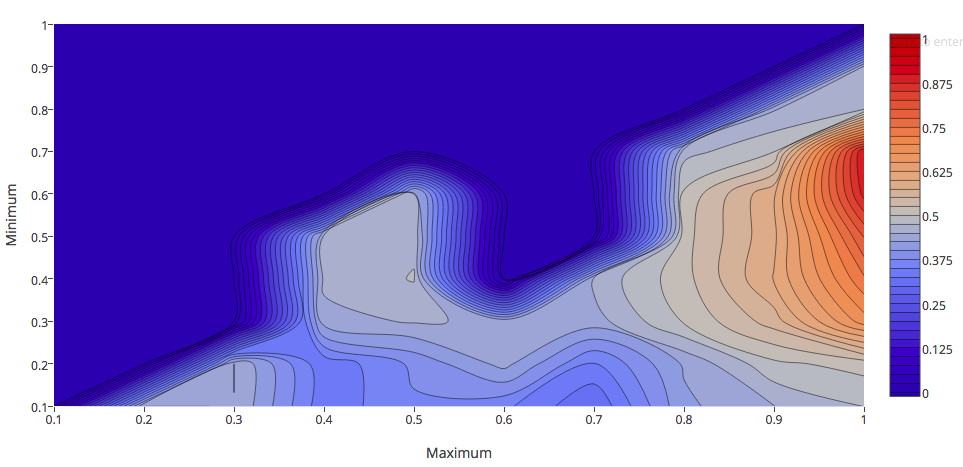
\includegraphics[scale=0.40]{img/ploty.png}
    \caption{Countour Plot of the minimum (y axis) and maximum (x axis) limits with 250 empty spaces}
\end{figure}

As we can see in Figure 1 there is obviously a limit (see \textbf{Figure 2}) where the segregation spikes only decreasing
when lowering the maximum limit. This is the threshold we were looking for.

By analysing the countour plot we can notice that if we fix the maximum limit at 100\% and increase the mininum limit when
it reaches 40\% the segregation increases sizably even though the agents don't mind being near 60\% of agents from other
race they choose to segregate themselves.

On the other hand when it reaches $0.75$ and above it becomes impossible to satisfy all the agents of a sample with 2
equiprobable races. For this values nothing can be concluded because when the agents can't be satisfied they remain moving
keeping the segregation at aproximatelly 50\%. This is only possible to assume because when generating the countour plot
it was used a sample population with 2 equiprobable races.

We also concluded that if we lower the maximum limit the segregation will be lower but it will be also more difficult to
satisfy all agents and will almost always exist some unsatisfied ones.

\begin{figure}[h!]
    \centering
    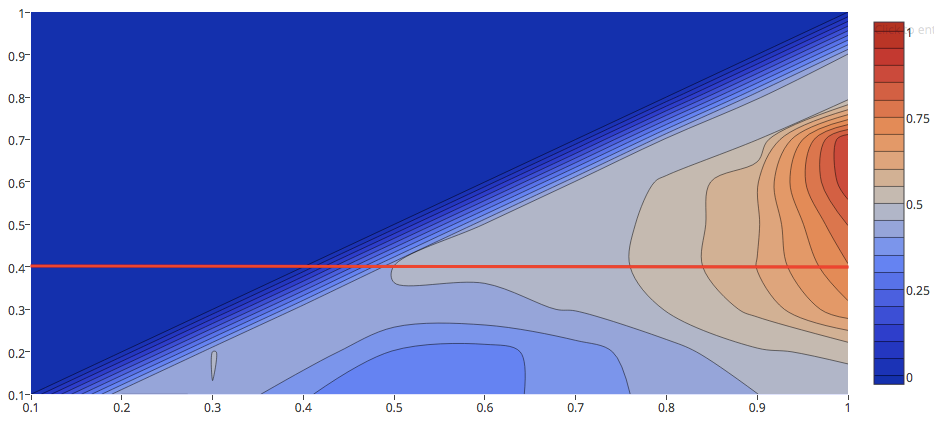
\includegraphics[scale=0.40]{img/ploty-a.png}
    \caption{Same Countour Plot of Figure 1 but with the minimum $0.4$ highlighted.}
\end{figure}

\newpage

\begin{figure}[h!]
    \centering
    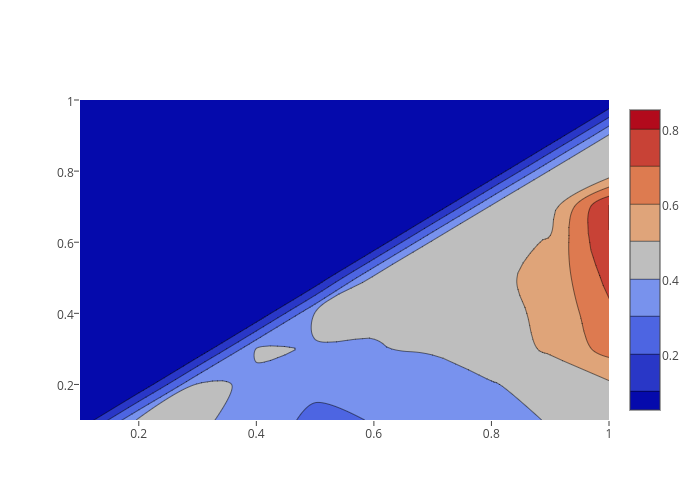
\includegraphics[scale=0.50]{img/500emptyspaces.png}
    \caption{Countour Plot of 2 races with 500 empty spaces}
\end{figure}

In this experience we modified the empty spaces from 250 to 500, to see if that would change the value of segregation. 

We can conclude that it didn't changed too much from our previous experience, maintaining an higher segregation near the minimum between 40\% and 70\% and the maximum at 90\%.

\newpage

\begin{figure}[h!]
    \centering
    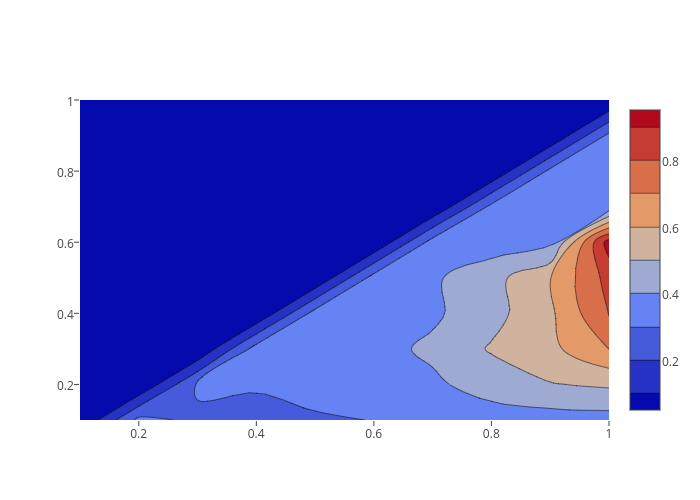
\includegraphics[scale=0.40]{img/3races75empty.png}
    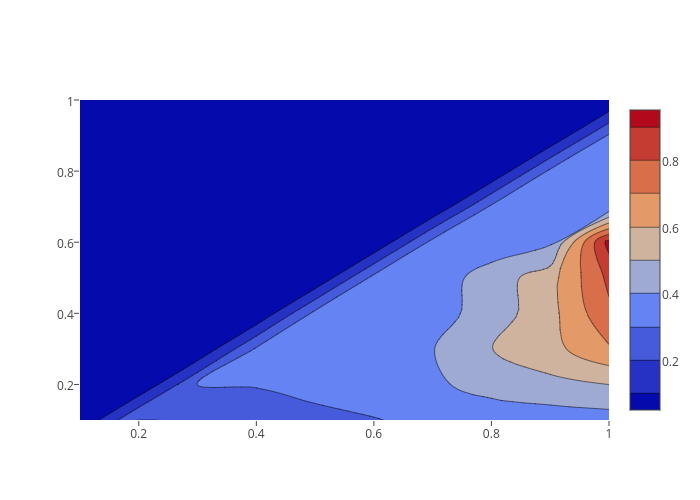
\includegraphics[scale=0.40]{img/3races150empty.png}
    \caption{Countour Plot of 3 races with 75 (top) and 150 (bottom) empty spaces}
\end{figure}

In this experience we changed the number of races from two to three and the empty spaces number to 75 and 150. 

In both experiences the results were similar and we verified that the segregation level is more continuous, passing through all the spectrum of values of segregation.

Relating the threshold we can say that with 3 races, the threshold is quite similar than with only 2 races but we can see that the segregation level reached a maximum value in this experience, reaching more than 0.9.

\newpage

\section{Reference}

\begin{description}
  \item[Python] \href{https://www.python.org}{www.python.org}
  \item[Tkinter] \href{https://wiki.python.org/moin/TkInter}{www.wiki.python.org/moin/TkInter}
  \item[plotly] \href{https://plot.ly/}{www.plot.ly}
  \item[Schelling's Model of Segregation] \href{http://nifty.stanford.edu/2014/mccown-schelling-model-segregation/}{www.nifty.stanford.edu/2014/mccown...}
  \item[Parable of the polygons: A playable post on the shape of society] \href{http://ncase.me/polygons/}{www.ncase.me/polygons}
\end{description}

\newpage

\end{document}
